\chapter{Outpost: A Lightweight Watchtower}  % Motivation
\label{chapter:outpost}

\section{Introduction}
As discussed in Chapter \ref{chap:intro},  Bitcoin limits the number of transactions that can fit into a block. The average size of a transaction is 300 bytes; with a block about every 10 minutes, the throughput is bounded to about 6 transactions per second. One may increase the block size and/or decrease the time between two blocks to achieve a higher throughput. However, these are consensus rule changes, and as such not easy to implement. Changing these parameters also adversely affect other security aspects of the Bitcoin network \cite{gervais2016security}.

Duplex Micropayment Channels \cite{decker_wattenhofer} and the Lightning Network \cite{poon_dryja} propose one type of solution to the scaling problem, allowing for higher throughput without changing Bitcoin's consensus rules. The idea of both these protocols is to handle most transactions outside the blockchain, in so-called channels. Bitcoin users would build a network of channels between them, and most transactions are handled in these channels. The Bitcoin blockchain would only be needed to setup and close these channels, and in this meta role, it handles far less transactions. 

The Lightning Network in particular has seen implementations from multiple teams of developers and researchers (LND \cite{lnd}, Eclair \cite{eclair}, Core-Lightning \cite{c_lightning}, LIT \cite{lit}), all implementing the same specifications \cite{bolt}. All of these implementations build node software that helps form a peer to peer network of payment channels where value denominated in Bitcoin can flow from node to node. 

However, there is still a major problem: Lightning channel payments can be received safely only if the receiving node stays online. Payment receivers risk losing payments if they go offline without closing channels that sent these payments, since a payment issuer can try to close a channel using an outdated earlier channel state. However, opening and closing channels are expensive blockchain transactions, which nodes want to avoid. To keep channels open \textit{and} be able to go offline, nodes need the services of so-called watchtowers \cite{watchtowers} to watch the Bitcoin blockchain and prevent fraudulent channel closures.

Watchtowers are \textit{always-online} services run by impartial parties, either for an altruistic motive (to see the Lightning Network succeed), or for a business motive (to get paid by the participant(s) of a channel). If we consider the business motive, watchtower services can be paid either per fraud detected, or simply for watching. Given that the Lightning protocol punishes frauds, we posit that it is better to pay watchtowers based on their actual cost of watching, which is directly proportional to the amount of data they have to store. This, in turn, depends on the number of channels they watch and the number of transactions that each of these channels have. On the other side, given that frauds are rare, we also need a mechanism which allows a watchtower to prove to channels that it is indeed doing its job. In our construction, after each transaction, the channel (one or both of its parties) sends the watchtower some data and fees. The watchtower, at any point in the future, can be asked for a proof by the channel that the watchtower was online as new Bitcoin blocks were mined and had access to this channel transaction data. This proof-scheme makes a pay-per-transaction scheme palatable to channel operators.

The watchtower's ability to perform its service depends on being able to watch the Bitcoin blockchain for a large number of transactions, with specific transaction IDs (or prefixes of IDs). Watchtower implementations need to have access to (and possibly store) this vast set of transaction IDs ($\texttt{txid}$'s) and accompanying data per $\texttt{txid}$ that contain information on what to do when a specific $\texttt{txid}$ shows up on the blockchain. LND's proof of concept implementation of watchtowers \cite{lnd_watchtower} requires around 300-350 additional bytes of storage per $\texttt{txid}$. A single watchtower could watch millions of channels and each channel could have billions of these micro-transactions. This places a large storage cost on the watchtower, as it has to store this 350 byte blob per transaction, for every transaction it knows about. 

We propose Outpost, a construction that reduces this overhead to 16 bytes of additional storage. We do this using a novel lightning channel structure that changes the commitment transactions. In particular, we encode the information of a possible future transaction $T_f$ in a present transaction $T_p$, so that $T_f$ spends the output of $T_p$ itself. This is non-trivial given how Bitcoin constructs and uses its $\texttt{txid}$'s. Outpost's reduction in storage costs will directly translate to the reduction in the operational cost of maintaining watchtowers. We believe that this will prompt more developers to run watchtowers, and thereby help the Lightning Network succeed.

\section{Background}
\subsection{Lightning Network}
The Lightning Network is a peer to peer network of nodes running the Lightning node software. Each peer is connected to other peers through a specific construct called a payment channel. A payment channel is opened with a Bitcoin transaction that commits UTXOs controlled by two parties into a single output that is now controlled by a multisig that both parties have to sign to be able to spend in a future transaction. This is called the opening transaction ($topen$). Once the payment channel is opened, the two parties exchange signed Bitcoin transactions between each other. In these signed transactions, the total value of $topen$ is allotted to each party depending on how the parties want value to flow between them. For example, if the payment channel was opened with 5 BTC from Alice and 10 BTC from Bob, a subsequent state might split the total 15 BTC of the channel so that Alice gets 7 BTC and Bob gets 8 BTC. This new split indicates a 2 BTC value flow from Bob to Alice, possibly for some goods or service that Bob received from Alice. This new division of $\texttt{topen}$'s balance is established by Alice and Bob by exchanging partially signed commitment transactions ($\texttt{ctx}$) with each other that they can sign themselves and broadcast later. At this point, the payment channel can also be closed with a closing transaction if both Alice and Bob agree to it. This is done by signing the multisig UTXO created by $\texttt{topen}$ and sending 7 BTC to Alice and 8 BTC to Bob. 

Typically, a channel is kept open by exchanging further $\texttt{ctx}$'s that change the division of the balance between Alice and Bob as more goods and services go from Alice to Bob or vice versa. Note that at any time, if either party goes permanently offline, the counterparty can sign and broadcast their latest $\texttt{ctx}$ to ``commit'' the latest state of the channel to the blockchain. The ability to unilaterally close the channel in case the other party goes offline makes this construction trustless. As a penalty for unilaterally closing the channel, the broadcasting party is made to wait for a timelock, whereas the counterparty (the one who might have gone offline) gets to spend their share of the channel instantly. This setup can be argued to be fair, because if a party broadcasts their $\texttt{ctx}$ even if the counterparty is online, they get their share of the balance, but have to wait to spend it. The counterparty does not have to wait in this case.

Importantly, a party can try to unilaterally close a channel with a $\texttt{ctx}$ (say, $\texttt{previous\_ctx}$) that is not the latest agreed upon $\texttt{ctx}$ (say, $\texttt{latest\_ctx}$). Every party potentially has many such $\texttt{previous\_ctx}$s in their storage going back all the way to the channel opening. This allows the dishonest party to cheat the honest counterparty by picking an old, more favorable $\texttt{previous\_ctx}$ from the past and broadcasting it. Lightning channels handle this cheating possibility by allowing $\texttt{latest\_ctx}$ to be exchanged only if they are also accompanied by ways of revoking the immediate $\texttt{previous\_ctx}$. This revocation is handled through a revocation key that can allot the entire channel balance to the victim's control. This gives both parties a strong incentive to be honest. In case Alice tries to cheat by publishing a $\texttt{previous\_ctx}$, Alice does not get her share of the channel balance immediately because it is timelocked, thereby giving Bob a time window to penalize this cheating $\texttt{previous\_ctx}$. Bob looks up its corresponding revocation key that he got from Alice earlier, and uses it to construct the so-called justice transaction ($\texttt{jtx}$) to penalize this $\texttt{previous\_ctx}$. To be able to detect cheating, Bob has to monitor the blockchain for all $\texttt{previous\_ctx}$s so that he can then construct the corresponding $\texttt{jtx}$ and broadcast it. This is possible only if Bob is online whenever a new Bitcoin block is mined. If Bob is offline, Alice can cheat Bob by broadcasting a $\texttt{previous\_ctx}$ that is more favorable to her than the current channel balance reflected in the $\texttt{latest\_ctx}$. 

\subsection{Watchtowers}

To be able to go offline, Bob enlists the help of a watchtower that is always online, and can monitor the blockchain for cheating $\texttt{ctx}$'s. Bob gives the watchtower the first 16 bytes of every $\texttt{ctx}$'s transaction ID ($\texttt{ctx\_txid}$), and encrypts the signed $\texttt{jtx}$ to get an encrypted blob ($\texttt{ejtx}$) using the other 16 bytes of $\texttt{ctx\_txid}$ as the encryption key. Bob gives the pair $\texttt{[ctx\_txid\_prefix, ejtx]}$ to the watchtower every time a new channel update is agreed upon. 

The watchtower stores a map, where keys are $\texttt{ctx\_txid\_prefixes}$ and values are $\texttt{ejtx}$s. It then watches the Bitcoin blockchain for any transaction whose $\texttt{txid\_prefix}$ matches any of the keys in its own map. If the watchtower finds a match, it extracts the $\texttt{txid\_suffix}$ from the blockchain $\texttt{txid}$, and uses this $\texttt{txid\_suffix}$ to decrypt the corresponding $\texttt{ejtx}$ from its map to get the raw $\texttt{jtx}$, which is already signed by the corresponding Bob of that channel. The watchtower then broadcasts this $\texttt{jtx}$ on the network to penalize the corresponding Alice of that channel. In implementations such as Lightning Network's LND \cite{lnd}, the watchtower is not made to store the entire signed $\texttt{jtx}$, but an encoded struct that has addresses, signatures, and other metadata to be able to construct the $\texttt{jtx}$. This encoded struct is smaller than the corresponding raw bitcoin transaction, but is still around 300-350 bytes. The $\texttt{ctx\_txid\_prefix}$ is constant at 16 bytes.

A single watchtower could be watching multiple channels and yet be oblivious to it. The watchtower just sees a stream of \sloppy $\texttt{[txid\_prefix, ejtx]}$ pairs that it has to store, possibly forever. Such a watchtower cannot identify channels from such a stream as there is no channel identifier in each pair. This design preserves channel privacy in the sense that a watchtower cannot identify how many channel updates any particular channel has had. As a side note, if a channel has been closed, channel participants have no standardized way of informing the watchtower that a set of $\texttt{[txid\_prefix, ejtx]}$ pairs can be deleted from the watchtower's global map. One possible way is for the watchtower to allocate a limit on storage per user, and use a FIFO order to delete older items from its storage.

\section{Outpost} %: Lightweight Watchtower Construction}
In this paper, we propose Outpost, a watchtower construction where it is possible to store the $\texttt{ejtx}$ inside the $\texttt{ctx}$ that is exchanged between Alice and Bob as a part of the channel update. In other words, we can store the ``future'' justice transaction in the ``present'' commitment transaction. If this is possible, the watchtower just has to store a map where keys are prefixes of $\texttt{ctx\_txid}$s and values are decryption keys for the corresponding $\texttt{ejtx}$. The $\texttt{ejtx}$ itself does not need to be stored by the watchtower as it is now available in the cheating $\texttt{ctx}$ that appears on the blockchain. With the Outpost construction, when a watchtower sees a cheating $\texttt{ctx}$ on the blockchain, the following happens:
\begin{enumerate}
\item The watchtower looks up the transaction in its global map, and finds the corresponding decryption key.
\item The watchtower extracts the $\texttt{ejtx}$ from the $\texttt{ctx}$ which was seen on the blockchain.
\item The watchtower uses the decryption key found in its map and decrypts $\texttt{ejtx}$ to get the pre-signed $\texttt{jtx}$.
\item The watchtower broadcasts this pre-signed $\texttt{jtx}$.
\end{enumerate}

\subsection{Why is this not possible in classic Lightning?}

For Alice and Bob to have a signed $\texttt{jtx}$ for a corresponding $\texttt{ctx}$, they need to first build the $\texttt{jtx}$ with its inputs and outputs. The outputs are straightforward. For the $\texttt{ctx}$ broadcast-able by Alice, the corresponding $\texttt{jtx}$ will send all of Alice's timelocked balance to Bob without any timelocks. The inputs are not so straightforward. To refer to $\texttt{ctx}$' outputs as the inputs for $\texttt{jtx}$, we need to have $\texttt{ctx\_txid}$. Let us say we have $\texttt{ctx\_txid}$, and use it construct a $\texttt{jtx}$, and get Alice and Bob to sign it. Alice then uses some encryption key and encrypts $\texttt{jtx}$ to get $\texttt{ejtx}$. We ``encode'' $\texttt{ejtx}$ in $\texttt{ctx}$ by using the \texttt{OP\_RETURN} technique and make it the 3rd output of $\texttt{ctx}$. Now, we have a self-loop problem, given that the $\texttt{ctx\_txid}$ is constructed by double SHA256 hashing the entire transaction, with its inputs and outputs. The moment we add a 3rd output, the $\texttt{ctx\_txid}$ present in $\texttt{ejtx}$ is not the real $\texttt{ctx\_txid}$. Given the way Bitcoin $\texttt{txid}$'s are constructed, there is no obvious way to encode a $\texttt{jtx}$ that spends $\texttt{ctx}$, and still encode this $\texttt{jtx}$ in the same $\texttt{ctx}$.

\subsection{Two other constructions that do not work}

\subsubsection{Data Drop Method}
One well known way of encoding arbitrary data in a Bitcoin transaction is to use the so-called Data-Drop method using P2SH transactions as elaborated in Sward et al \cite{sward2018data}. To encode $\texttt{jtx}$ inside $\texttt{ctx}$, we split $\texttt{ctx}$ into two: $\texttt{ctx\textsubscript{1}}$ and $\texttt{ctx\textsubscript{2}}$. $\texttt{ctx\textsubscript{1}}$'s output can be locked with scriptPubKey:
\begin{verbatim}
OP_HASH160 <hash(redeem_script)> OP_EQUAL
\end{verbatim}

This will allow us to have a followup $\texttt{ctx\textsubscript{2}}$ whose scriptSig has a redeem script of the type:
\begin{verbatim}
OP_DROP 2 <alice_pubkey> <bob_pubkey>
2 OP_CHECKMULTSIG
\end{verbatim}

And scriptSig of the type:
\noindent
\begin{verbatim}
0 <alice_sig> <bob_sig> <ejtx> <redeem_script>
\end{verbatim}

With this setup, we can include arbitrary data in the scriptSig between the signatures and the actual redeem script, and encode $\texttt{jtx}$ in this data (shown as $\texttt{ejtx}$ above). The problem with this approach is that anyone can tamper with the scriptSig in such a way that this arbitrary data is changed, and the redeem script is still valid (scriptSig malleability). There is no guarantee that $\texttt{ctx\textsubscript{2}}$ will make it to the blockchain in such a way that $\texttt{ejtx}$ can be read off of it. Any intercepting forwarding full node, or even the miner who mines the relevant block can change the transaction to drop this extra data.

\subsubsection{Data Hash Method}
\sloppy
Another way of encoding arbitrary data in a Bitcoin transaction that is immune to scriptSig malleability is using the so-called Data-Hash method using P2SH transactions; also elaborated in Sward et al\cite{sward2018data}. Here, like with the data-drop method, $\texttt{ctx}$ is split into $\texttt{ctx\textsubscript{1}}$ and $\texttt{ctx\textsubscript{2}}$, and have $\texttt{ctx\textsubscript{1}}$'s output locked in the same way as before. We prevent the subsequent $\texttt{ctx\textsubscript{2}}$'s scriptSig from being tampered with, by encoding $\texttt{ejtx}$ in the redeem script, and then using this redeem script's hash in $\texttt{ctx\textsubscript{1}}$. Say, $\texttt{ctx\textsubscript{2}}$'s redeem script looks like this: 
\begin{verbatim}
OP_HASH160 <hash(ejtx)> OP_EQUALVERIFY
2 <alice_pubkey> <bob_pubkey> 2 OP_CHECKMULTSIG
\end{verbatim}

$\texttt{ctx\textsubscript{2}}$'s scriptSig will encode $\texttt{ejtx}$ in the same way as before. This will enforce that the scriptSig cannot be tampered with while still keeping $\texttt{ctx\textsubscript{2}}$ valid. If any tampering of $\texttt{ctx\textsubscript{2}}$'s scriptSig (which contains $\texttt{ejtx}$) happens en route to a mined block, $\texttt{ctx\textsubscript{2}}$ is not valid anymore as it cannot spend what $\texttt{ctx\textsubscript{1}}$ locks. The data hash method solves the scriptSig malleability issue. 

There is a subtler self-loop problem though: we include $\texttt{ejtx}$ in the redeem script of $\texttt{ctx\textsubscript{2}}$, and the redeem script's hash in $\texttt{ctx\textsubscript{1}}$. This changes the $\texttt{txid}$ of $\texttt{ctx\textsubscript{1}}$ and we have to spend $\texttt{ctx\textsubscript{1}}$ (through $\texttt{ctx\textsubscript{2}}$) in $\texttt{ejtx}$. We are back to the self-loop problem again, where we have to spend a UTXO in the future, but also encode the spending transaction in the present. The moment we do the encoding, the future UTXO's input $\texttt{txid}$ changes, thereby invalidating the encoding. With a linear chain of transactions with the child spending the parents' output, we run into this self-loop problem. In the following section, we show how to encode the future in the present by doing it in a separate transaction path, and then merging these paths later.

\subsection{Split Commitment Transaction Construction}
In Outpost, we have 3 commitment transactions that represent a single channel state, as opposed to just 1 commitment transaction in classic Lightning. This is in addition to the opening transaction and the justice transaction. In this section, $\texttt{topen}$ is common to both parties, Alice and Bob. Without loss of generality, the other 3 commitment transactions and 1 justice transaction are assumed to be Alice's to broadcast. Bob has symmetrically opposite transactions that he holds. Another convention in the following listings is that $pubkey\_i$ can be signed by $sig\_i$. In Section \ref{protocol}, we define these transactions more precisely with respect to signing, holding (not \textit{hodling}), and broadcasting.
\subsubsection{Opening Transaction}
$\texttt{topen}$ is exactly the same as in classic Lightning, in the sense that it has to spend two UTXOs, one of which is owned by Alice and one by Bob. 

\begin{lstlisting}[
    basicstyle=\ttfamily\small,
    caption={Opening Transaction in Bitcoin Script-like pseudocode},
    label=topen
]
TOPEN: {
 txid: TOPEN_TXID
 vin: [{
   txid: source TXN that pays Alice
   scriptSig: <Alice sig_0>
  },{     
   txid: source TXN that pays Bob
   scriptSig: <Bob sig_0>
  }]      
 vout: [{
   value: <value of the channel>
   scriptPubKey: 
        2 
        <Alice pubkey_1> 
        <Bob pubkey_1> 
        2 OP_CHECKMULTISIG
  }]}
\end{lstlisting}

\subsubsection{Commitment Transaction 1}
The output of $\texttt{topen}$ is spendable by $\texttt{ctx\textsubscript{1}}$ (see Listing \ref{ctx1}), which is similar to classic Lightning's commitment transaction, but differs in a few important ways.
\begin{enumerate}
    \item Output at index 0: Alice's balance is \textit{not} spendable by just Alice after a timelock (as in classic Lightning). It is spendable with a multisig that both Alice and Bob need to sign. This allows us to ``fork'' this output into either the justice transaction or a followup commitment transaction ($\texttt{ctx\textsubscript{2}}$). This $\texttt{ctx\textsubscript{2}}$ gives Alice's share to Alice, but guards it with a timelock. This way, we realize classic Lightning's key idea that the broadcaster's balance needs to be timelocked to allow the counterparty to react in time.
    \item Output at index 1: As in classic Lightning, Bob's part is immediately spendable (no timelock) by Bob with just his signature.
    \item Output at index 2: The \textit{auxiliary} output, which can be spent with a signature by both Alice and Bob, but has a value that is insignificant - say, just enough to be spendable with minimal fees. The sole purpose of the auxiliary output is to be a part of a subsequent auxiliary transaction ($\texttt{aux\_ctx}$) which encodes $\texttt{ejtx}$. Its need will become more clear in the subsequent paragraphs.
\end{enumerate}

\begin{lstlisting}[
    mathescape=true,
    basicstyle=\ttfamily\small,
    caption={Commitment Transaction 1 in Bitcoin Script-like pseudocode},
    label=ctx1
]
CTX_1: {
 txid: CTX_1_TXID
 vin: [{
   txid: TOPEN_TXID
   index: 0
   scriptSig: 
        0 <Alice sig_1> <Bob sig_1>
  }]
 vout: [{
   value: <Alice balance>
   scriptPubKey:
            2 
            <Alice pubkey_2> 
            <Bob pubkey_2> 
            2 OP_CHECKMULTISIG
  }, {
   value: <Bob balance>
   scriptPubKey: 
        <Bob pubkey_3> OP_CHECKSIG
  }, {
   value: INSIGNIFICANT_VALUE ($\epsilon$)
   scriptPubKey: 
        2 
        <Alice pubkey_4> 
        <Bob pubkey_4> 
        2 OP_CHECKMULTISIG
  }]}
\end{lstlisting}

\subsubsection{Justice Transaction}
The $\texttt{jtx}$ (see Listing \ref{jtx}) spends the multisig output of $\texttt{ctx\textsubscript{1}}$ and gives all of Alice's share to Bob. Note that Alice will sign this transaction only after Bob signs it, and will not hand it over to Bob in raw format. Alice encrypts this $\texttt{jtx}$ with a key of her choice to derive $\texttt{ejtx}$ and hands over $\texttt{ejtx}$ to Bob by encoding it in $\texttt{aux\_ctx}$. 

\begin{lstlisting}[
    basicstyle=\ttfamily\small,
    caption={Justice Transaction in Bitcoin Script-like pseudocode},
    label=jtx
]
JTX: {
 txid: JTX_TXID
 vin: [{
   txid: CTX_1_TXID
   index : 0
   scriptSig: 
        0 <Alice sig_2> <Bob sig_2>
  }],
 vout: [{
   value: <Alice balance>
   scriptPubKey: 
        <Bob pubkey_5> OP_CHECKSIG
  }]}
\end{lstlisting}

\subsubsection{Auxiliary Commitment Transaction}
The purpose of $\texttt{aux\_ctx}$ (see Listing \ref{aux_ctx}) is to be a vehicle to encode the encrypted justice transaction ($\texttt{ejtx}$) as its ``non-monetary'' \texttt{OP\_RETURN} output. We inject $\texttt{aux\_ctx}$ in the channel by making it spend the small insignificant value from $\texttt{ctx\textsubscript{1}}$, and make the final transaction $\texttt{ctx\textsubscript{2}}$ spend from $\texttt{aux\_ctx}$'s ``monetary'' output. This way, the channel cannot be closed unilaterally without broadcasting $\texttt{aux\_ctx}$. Once it is broadcast, $\texttt{ejtx}$ is visible on the blockchain and anyone with a key to decrypt it can get the signed raw $\texttt{jtx}$ and can broadcast it.

\begin{lstlisting}[
    mathescape=true,
    basicstyle=\ttfamily\small,
    caption={Auxiliary CTX in Bitcoin Script-like pseudocode},
    label=aux_ctx
]
AUX_CTX: {
 txid: AUX_CTX_TXID
 vin: [{
   txid: CTX_1_TXID
   index: 2
   scriptSig: 
        0 <Alice sig_4> <Bob sig_4>
  }]
 vout: [{
   value: INSIGNIFICANT_VALUE ($\epsilon$)
   scriptPubKey: 
        2 
        <Alice pubkey_6> <Bob pubkey_6> 
        2 
        OP_CHECKMULTISIG
  }, {
   value: 0
   scriptPubKey: OP_RETURN EJTX
  }]}
\end{lstlisting}

\subsubsection{Commitment Transaction 2}
The final piece of the puzzle is $\texttt{ctx\textsubscript{2}}$ (see Listing \ref{ctx2}). It spends outputs of both $\texttt{ctx\textsubscript{1}}$ (the actual channel balance carrying commitment) and $\texttt{aux\_ctx}$ (the $\texttt{ejtx}$ carrying commitment). These outputs make up the inputs of $\texttt{ctx\textsubscript{2}}$, and are timelocked using BIP68 \cite{BIP68} sequence numbers. In Listing \ref{ctx2}, we use a delay of 144 blocks (1 day), which is represented as 0x00000090. The consensus rules of Bitcoin do not let this transaction through till 144 blocks have passed since both $\texttt{ctx\textsubscript{1}}$ and $\texttt{aux\_ctx}$ are confirmed. This gives the watchtower enough time to look for a cheating $\texttt{aux\_ctx}$ on the blockchain, and decrypt $\texttt{ejtx}$ which is visible in $\texttt{aux\_ctx}$. As a part of the protocol (refer \ref{protocol}), Alice would have shared with Bob the decryption key for $\texttt{ejtx}$ in a followup state. Subsequently, Bob would have given this key, along with $\texttt{ctx\textsubscript{1}\_txid}$ to the watchtower. This ensures that the watchtower has everything it needs to construct $\texttt{jtx}$ and broadcast it without Bob ever having to be online. 

Note that if $\texttt{jtx}$ is confirmed on the Bitcoin blockchain, $\texttt{ctx\textsubscript{2}}$ becomes invalid as one of its inputs ($\texttt{ctx_1}$'s output number \#0) has now been consumed. 

\begin{lstlisting}[
    basicstyle=\ttfamily\small,
    caption={Commitment Transaction 2 in Bitcoin Script-like pseudocode},
    label=ctx2
]
CTX_2: {
 txid: CTX_2_TXID
 vin: [{
   txid: CTX_1_TXID
   index: 0
   scriptSig: 
        0 <Alice sig_2> <Bob sig_2>
        OP_TRUE
   sequence: 0x00000090
  },{
   txid: AUX_CTX_TXID
   index: 0
   scriptSig: 
        0 <Alice sig_6> <Bob sig_6>
   sequence: 0x00000090
  }]
 vout: [{
   value: <Alice balance>
   scriptPubKey: 
        <Alice pubkey_7> OP_CHECKSIG
  }]}
\end{lstlisting}

\subsubsection{Cooperative Closure}
If Alice and Bob are done using their channel, and want to get their current balances out, they create a classic Lightning like closure transaction that spends $\texttt{topen}$ and allocates balances to Alice and Bob based on the latest state of the channel. With respect to opening and closing a channel, Outpost's transactions on the blockchain will look exactly the same as in classic Lightning. Listing \ref{closure2} shows a cooperative closure.

\begin{lstlisting}[
    basicstyle=\ttfamily\small,
    caption={Cooperative closure in Bitcoin Script-like pseudocode},
    label=closure2
]
CLOSURE: {
 txid: CLOSURE_TXID
 vin: [{
   txid: TOPEN_TXID
   index: 0
   scriptSig: 
        0 <Alice sig_1> <Bob sig_1>
  }]
 vout: [{
   value: <Alice balance>
   scriptPubKey: 
        <Alice pubkey_8> OP_CHECKSIG
  }, {
   value: <Bob balance>
   scriptPubKey: 
        <Bob pubkey_8> OP_CHECKSIG
  }]}
\end{lstlisting}


\subsubsection{Cheating}
If Alice cheats by broadcasting an earlier state in the form of $\texttt{ctx\textsubscript{1}}$, $\texttt{aux\_ctx}$, and $\texttt{ctx\textsubscript{2}}$ to the network, $\texttt{ctx\textsubscript{1}}$ and $\texttt{aux\_ctx}$ can be mined and confirmed immediately, but $\texttt{ctx\textsubscript{2}}$ is timelocked. In the timelocked time, the watchtower can watch for $\texttt{aux\_ctx}$ on the Bitcoin blockchain, extract and decrypt $\texttt{ejtx}$ from it to get $\texttt{jtx}$ and broadcast $\texttt{jtx}$, thereby invalidating $\texttt{ctx\textsubscript{2}}$, and also giving Bob the entire channel balance.

\subsubsection{Unilateral Closure}
If Bob goes offline, and Alice wants to unilaterally close the channel (not cheating), she broadcasts the current state in the form of $\texttt{ctx\textsubscript{1}}$, $\texttt{aux\_ctx}$, and $\texttt{ctx\textsubscript{2}}$. She knows that the decryption key for $\texttt{ejtx}$ from the current state has not been shared with Bob, and hence, not with any watchtower either. This makes Alice get back her side of the balance, but after a timelock. This tradeoff of the unilateral channel closure having to wait for timelocks to expire is the key design insight of classic Lightning, and we preserve the same principle, but through BIP68 input locks in $\texttt{ctx\textsubscript{2}}$.

\subsubsection{Griefing}
Griefing refers to a class of attacks where the attacker does not want to make a profit, but puts the counterparty at a disadvantage by deviating from the protocol. In our protocol, the watchtower can only help if both $\texttt{ctx\textsubscript{1}}$ and $\texttt{aux\_ctx}$ are on the blockchain. Alice can initiate a griefing attack when Bob is offline by broadcasting a $\texttt{ctx\textsubscript{1}}$ from an older state and \textit{not} broadcasting the corresponding $\texttt{aux\_ctx}$ and $\texttt{ctx\textsubscript{2}}$. Note that Alice is not cashing out here, but the watchtower cannot help Bob either - because $\texttt{aux\_ctx}$ is not published on the blockchain.

This attack is possible because $topen$ has been spent by $\texttt{ctx\textsubscript{1}}$, and has created a UTXO that cannot be spent by Bob alone. We can mitigate this by adding a flow to $\texttt{ctx\textsubscript{1}}$ such that the UTXO it creates can be spent by Bob after a timelock unless it is spent by $\texttt{aux\_ctx}$. This incentivizes Alice to not publish just $\texttt{ctx\textsubscript{1}}$. If she does that, and does not publish the corresponding $\texttt{aux\_ctx}$ and $\texttt{ctx\textsubscript{2}}$, the entire channel balance can be swept by Bob after this timelock expires. Note that this timelock has to be larger than the timelock in $\texttt{ctx\textsubscript{2}}$. 

\begin{figure}[H]
\begin{centering}
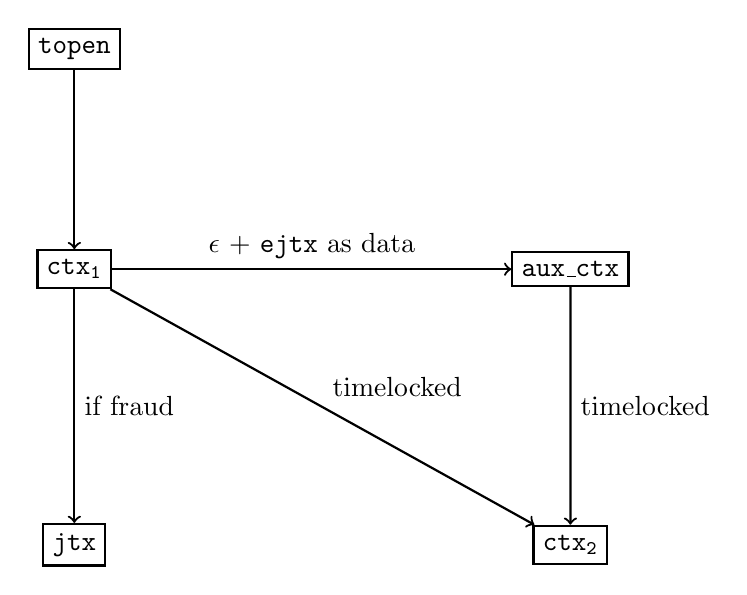
\begin{tikzpicture}
  [scale=.7,auto=left]
  \node[rectangle, draw, thick] (topen) at (1,10) {$\texttt{topen}$};
  \node[rectangle, draw, thick] (ctx_1) at (1,6)  {$\texttt{ctx\textsubscript{1}}$};
  \node[rectangle, draw, thick] (aux_ctx) at (10,6) {$\texttt{aux\_ctx}$};
  \node[rectangle, draw, thick] (ctx_2) at (10,1)  {$\texttt{ctx\textsubscript{2}}$};
  \node[rectangle, draw, thick] (jtx) at (1,1)  {$\texttt{jtx}$};
  
  \draw[thick, ->] (topen) -- node[draw=none,fill=none] {} (ctx_1);
  \draw[thick, ->] (ctx_1) -- node[draw=none,fill=none] {$\epsilon$ + $\texttt{ejtx}$ as data} (aux_ctx);
  \draw[thick, ->] (ctx_1) -- node[draw=none,fill=none] {timelocked} (ctx_2);
  \draw[thick, ->] (aux_ctx) -- node[draw=none,fill=none] {timelocked} (ctx_2);
  \draw[thick, ->] (ctx_1) -- node[draw=none,fill=none] {if fraud} (jtx);
\end{tikzpicture}
\caption{Transaction Flow}
\label{transaction_flow}
\end{centering} 
\end{figure}

\section{Protocol} \label{protocol}
In this section, we elaborate on how, at each stage of the protocol, transactions are signed and exchanged by Alice and Bob. Decryption keys of encrypted blobs are also exchanged as a part of the protocol.

During channel opening, as with classic Lightning, Alice and Bob construct a single $\texttt{topen}$ using their own inputs, and make it spendable by a multisig that they both need to sign. Note that between both Alice and Bob, there is only one $\texttt{topen}$. Alice and Bob do not sign this $\texttt{topen}$ before the follow-up transactions of the next step ($\texttt{ctx\textsubscript{1}}$, $\texttt{aux\_ctx}$, and $\texttt{ctx\textsubscript{2}}$) have been exchanged. This ensures that if either party disappears after the signed $\texttt{topen}$ has been broadcast, the other party is not held in limbo and can close the channel unilaterally. In the following protocol description, we use ``alice'' and ``bob'' superscripts to denote the transactions that are held by Alice and Bob. In Lightning channels, both parties keep symmetric transactions to represent the collective state. 

\subsection{Opening Transaction}
\subsubsection{$Bob\,\to\,Alice$}
\begin{itemize}[leftmargin=4\parindent]
    \item A UTXO that Bob controls.
    \item Pubkeys that are required for followup transactions.
\end{itemize}
\subsubsection{$Alice\,\to\,Bob$}
\begin{itemize}[leftmargin=4\parindent]
    \item $\texttt{topen}$ with Alice's own UTXO filled in. This $\texttt{topen}$ has its multisig output filled in with one of Bob's pubkeys and one of Alice's own pubkeys. This $\texttt{topen}$ is not signed by either Alice or Bob yet.
    \item Two versions of $\texttt{ctx\textsubscript{1}}$ ($\texttt{ctx\textsubscript{1}\textsuperscript{alice}}$, $\texttt{ctx\textsubscript{1}\textsuperscript{bob}}$) which share the same input transaction $\texttt{topen}$. These two $\texttt{ctx\textsubscript{1}}$s have three outputs each. In $\texttt{ctx\textsubscript{1}\textsuperscript{alice}}$, the \nth{2} singlesig output is sent to Bob's pubkey. In $\texttt{ctx\textsubscript{1}\textsuperscript{bob}}$, the \nth{2} singlesig output is sent to Alice's pubkey. Note that Alice can construct both $\textt{ctx\textsubscript{1}}$s at this stage, and can even sign for her part of the input ($\texttt{topen}$) of each $\texttt{ctx\textsubscript{1}}$.
\end{itemize}
\subsubsection{$Bob\,\to\,Alice$}
\begin{itemize}[leftmargin=4\parindent]
    \item $\texttt{ctx\textsubscript{1}\textsuperscript{alice}}$ signed by Bob. Bob signs $\texttt{ctx\textsubscript{1}\textsuperscript{bob}}$ and keeps it for himself.
    \item $\texttt{jtx\textsuperscript{bob}}$ with Alice's balance sent to Bob's pubkey. Bob signs $\texttt{jtx\textsuperscript{bob}}$ without worry because its output is being sent to him.
\end{itemize}
\subsubsection{$Alice\,\to\,Bob$}
\begin{itemize}[leftmargin=4\parindent]
    \item $\texttt{jtx\textsuperscript{alice}}$ with Bob's balance sent to Alice's pubkey. Alice signs $\texttt{jtx\textsuperscript{alice}}$ without worry because its output is being sent to her.
    \item $\texttt{aux\_ctx\textsuperscript{bob}}$: Alice constructs the full signed $\texttt{jtx\textsuperscript{bob}}$ with her own signature, and encrypts it with a random key to derive $\texttt{ejtx\textsuperscript{bob}}$. She then constructs $\texttt{aux\_ctx\textsuperscript{bob}}$ with two outputs, one of which is the \texttt{OP\_RETURN} prefixed $\texttt{ejtx\textsuperscript{bob}}$. Alice signs $\texttt{aux\_ctx\textsuperscript{bob}}$ and sends it to Bob. After getting $\texttt{aux\_ctx\textsuperscript{bob}}$ signed by Alice, Bob signs it as well, but keeps it for himself.
    \item $\texttt{ctx\textsubscript{2}\textsuperscript{bob}}$: Alice also constructs the signed $\texttt{ctx\textsubscript{2}\textsuperscript{bob}}$, which needs her signatures for both its inputs: $\texttt{ctx\textsubscript{1}\textsuperscript{bob}}$ and $\texttt{aux\_ctx\textsuperscript{bob}}$. When Bob gets $\texttt{ctx\textsubscript{2}\textsuperscript{bob}}$ signed by Alice, he signs it and keeps it for himself.
\end{itemize}
\subsubsection{$Bob\,\to\,Alice$}
\begin{itemize}[leftmargin=4\parindent]
    \item $\texttt{aux\_ctx\textsuperscript{alice}}$: Bob constructs the fully signed $\texttt{jtx\textsuperscript{alice}}$ with his own signature, and encrypts it with a random key to derive $\texttt{ejtx\textsuperscript{alice}}$. He then constructs $\texttt{aux\_ctx\textsuperscript{alice}}$ with two outputs, one of which is the \texttt{OP\_RETURN} prefixed $\texttt{ejtx\textsuperscript{alice}}$. Bob signs $\texttt{aux\_ctx\textsuperscript{alice}}$ and sends it to Alice. After getting $\texttt{aux\_ctx\textsuperscript{alice}}$ signed by Bob, Alice signs it as well, but keeps it for herself.
    \item $\texttt{ctx\textsubscript{2}\textsuperscript{alice}}$: Bob also constructs the signed $\texttt{ctx\textsubscript{2}\textsuperscript{alice}}$, which needs his signatures for both its inputs: $\texttt{ctx\textsubscript{1}\textsuperscript{alice}}$ and $\texttt{aux\_ctx\textsuperscript{alice}}$. When Alice gets $\texttt{ctx\textsubscript{2}\textsuperscript{alice}}$, she signs it and keeps it for herself.     
    \item $\texttt{topen}$: At this point, Bob has all the followup transactions signed by Alice with him, and can safely sign $\texttt{topen}$.
\end{itemize}
\subsubsection{$Alice\,\to\,Blockchain$}
\begin{itemize}[leftmargin=4\parindent]
    \item $\texttt{topen}$: At this point, Alice has all the followup transactions signed by Bob with her, and can safely sign $\texttt{topen}$ and broadcast it on the Bitcoin network.
\end{itemize}

\subsection{State Update}
\subsubsection{$Bob\,\to\,Alice$}
\begin{itemize}[leftmargin=4\parindent]
    \item Same as from the Opening Transaction, except for the UTXO part.
\end{itemize}
\subsubsection{$Alice\,\to\,Bob$}
\begin{itemize}[leftmargin=4\parindent]
\item Same as from Opening Transaction, except for the $\texttt{topen}$ part.
\end{itemize}
\subsubsection{$Bob\,\to\,Alice$}
\begin{itemize}[leftmargin=4\parindent]
    \item Same as from Opening Transaction.
\end{itemize}
\subsubsection{$Alice\,\to\,Bob$}
\begin{itemize}[leftmargin=4\parindent]
    \item Same as from Opening Transaction.
\end{itemize}
\subsubsection{$Bob\,\to\,Alice$}
\begin{itemize}[leftmargin=4\parindent]
    \item Same as from Opening Transaction.
    \item Decryption Key: At this point, Bob has all the followup transactions signed by Alice with him and has effectively moved to the next state. He can now let Alice decrypt the previous state's $\texttt{ejtx\textsuperscript{bob}}$ if it is ever seen on the blockchain (through the confirmation of $\texttt{aux\_ctx\textsuperscript{bob}}$). To do that, Bob sends Alice the key that can decrypt $\texttt{ejtx\textsuperscript{bob}}$ from the previous state. Now, Alice can send $\texttt{aux\_ctx\textsuperscript{alice}}$'$s$ $\texttt{txid}$ and this decryption key to the watchtower.
\end{itemize}
\subsubsection{$Alice\,\to\,Bob$}        
\begin{itemize}[leftmargin=4\parindent]
    \item Decryption Key: At this point, Alice has all the followup transactions signed by Bob with her and has effectively moved to the next state. She can now let Bob decrypt the previous state's $\texttt{ejtx\textsuperscript{alice}}$ if it is ever seen on the blockchain (through the confirmation of $\texttt{aux\_ctx\textsuperscript{alice}}$). To do that, Alice sends Bob the key that can decrypt $\texttt{ejtx\textsuperscript{alice}}$ from the previous state. Now, Bob can send $\texttt{aux\_ctx\textsuperscript{bob}}$'$s$ $\texttt{txid}$ and this decryption key to a possibly different watchtower.
\end{itemize}

\section{Limitations}
\subsection{\texttt{OP\_RETURN} size limit}
One key limitation of the Outpost construction is the size constraint on the \texttt{OP\_RETURN} output in $\texttt{aux\_ctx}$. This size limitation is enforced by the IsStandard function of Bitcoin Core's reference implementation, which drops any transaction that has an \texttt{OP\_RETURN} output of more than 80 bytes. This rule is not enforced by the Bitcoin consensus mechanism, in the sense that transactions with such outputs are considered valid, but not standard. Miners who see these transactions can still add them to their block template and generate valid blocks with them. So, $\texttt{aux\_ctx}$ can have the \texttt{OP\_RETURN} output we want and can be handed to the miners directly to be included in their block template without violating Bitcoin's consensus rules. 

Another way to circumvent this size limit is to use the data-hash method from \cite{sward2018data} to encode arbitrary data in a standard Bitcoin transaction. In our case, we have to split $\texttt{aux\_ctx}$ into two transactions, say $\texttt{aux\_ctx\textsubscript{1}}$ and $\texttt{aux\_ctx\textsubscript{2}}$. In $\texttt{aux\_ctx\textsubscript{1}}$, there will be a hash of a specific redeem script (thereby making $\texttt{aux\_ctx\textsubscript{1}}$ a P2SH transaction). The actual redeem script will be in $\texttt{aux\_ctx\textsubscript{2}}$ and will enable the scriptSig of $\texttt{aux\_ctx\textsubscript{2}}$ to have the encrypted payload. The payload in our case is a typical $\texttt{jtx}$ that spends using a multisig and pays to a P2PKH address. With signatures, these transactions are typically $\sim$350 bytes long. They can be encrypted with AES-128 and we get an $\texttt{ejtx}$ of size $\sim$360 bytes. This can be encoded in the scriptSig of $\texttt{aux\_ctx\textsubscript{2}}$ quite easily as the maximum script element size in Bitcoin is 520 bytes.

\subsection{Transaction Bloat and Complexity}
In the Outpost construction, instead of one $\texttt{ctx}$ per party to handle the channel update, like in classic Lightning, we have 3 transactions per party per state. This is not a true limitation, in that we are not increasing storage cumulatively. Each party needs to just keep their latest state in storage, and can discard all previous states. So, storing one transaction in classic Lightning vs three transactions with Outpost should not matter a lot. In classic Lightning, each party has to store the $\texttt{ctx\_txid}$ of each $\texttt{ctx}$ that its counter-party can broadcast, to watch for cheating transactions. Along side the $\texttt{ctx\_txid}$, the party has to also store the revocation key needed to construct the $\texttt{jtx}$ for a cheating $\texttt{ctx}$. In Outpost, each party has to store the $\texttt{ctx\textsubscript{1}\_txid}$ of each $\texttt{ctx\textsubscript{1}}$ that its counter-party has to broadcast to cheat. Along side the $\texttt{ctx\textsubscript{1}\_txid}$, the party has to also store the decryption key for the encoded $\texttt{ejtx}$ inside the $\texttt{aux\_ctx}$. At the node level, this extra storage requirement is the same in Outpost as in classic Lightning. But at the watchtower level, it leads to considerable savings, which we will explore in the Analysis section.

\section{Optimization}
Each party can derive their $\texttt{jtx}$ encryption keys independently of each other, forcing the counter-party to store these decryption keys independently. We can optimize some of this storage away by deriving encryption keys using a hash-chain or an encrypted-key-chain. Say, Alice wants to generate 1000 encryption keys such that they can be used in a payment channel with Bob - with one key being used for each state update. As state updates happen, Alice will give Bob these keys one by one, and Bob has to store all of them, along with the $\texttt{ctx\textsubscript{1}\_txid}$ for each key. This can be made more efficient if Bob can just store the most recent key he received from Alice, but can compute the other keys based on this latest key. 

There are multiple schemes that Alice could use to generate encryption keys such that if $K_i$ and $K_{i+1}$ are two keys with timestamps $\mathit{i}$ and $i+1$, then:
\begin{itemize}
\item It is easy for Alice to generate either key from the other.
\item It is hard for Bob to generate $K_{i+1}$ from $K_i$, but easy to generate $K_i$ from $K_{i+1}$. 
\end{itemize}
We briefly outline 2 such schemes:
\begin{itemize}
    \item Alice pre-generates these keys by starting with one random key, and generating subsequent keys by hashing the previous key, say using SHA256 - thereby forming a hash-chain. She starts her channel with Bob by using the last such generated key, and at each followup state, uses the hash preimage (which is also a hash of its own preimage) as the next key. Bob can now discard old keys as new keys come along, as he can always reconstruct them using the commonly known one-way hash function if he knows the current key and the index number of what key he wants to reconstruct. This scheme needs Alice to pre-compute hashes and store them on the ``forward chain'', thereby incurring both computation and storage costs. Going on the ``backwards chain'' is a matter of trivial lookup. A more advanced version of this scheme is found in \cite{shachain}.
    \item Alice creates an RSA key pair of sufficient length (say, modulus of size 2048 bits), keeps the private key to herself, and shares the public key with Bob. Say, $\mathit{e}$ and $\mathit{n}$ are the exponent and the modulus components of the public key, Alice can start the key chain with a large random number in the range $\mathit{[2, n-1)}$ and decrypt it using the private key to generate the next key in the sequence. Note that every number in the range $\mathit{[2, n-1)}$ has a valid RSA decryption. A secure one-way hash function can be used as a key derivation function on this large number to generate the (smaller) symmetric key required to encrypt $\texttt{jtx}$ to get $\texttt{ejtx}$. Bob can always go back the chain and find older keys by encrypting the latest key using the public key that he knows, but cannot create newer keys, as it requires decrypting the latest key.
\end{itemize}

We can even optimize away the need to store $\texttt{ctx\textsubscript{1}\_txid}$ for each state update. We can embed a channel ID in either $\texttt{ctx\textsubscript{1}}$ or $\texttt{aux\_ctx}$ which we can then watch for on the blockchain. We also need to track the index of the state to be able to derive the right decryption key to construct the necessary $\texttt{jtx}$. The channel ID and the index together can be stored as the \nth{4} output of $\texttt{ctx\textsubscript{1}}$ in an \texttt{OP\_RETURN} instruction. This gives us constant storage per channel with respect to what we have to watch for on the blockhain. All we need to store per channel is the channel ID and seed of the hash-chain. 

Using either of the schemes above, Bob's storage savings can also be realized at the watchtower level, if Bob is willing to let the watchtower know that all of his state updates are from the same channel by providing a channel ID in each of his watchtower requests. The watchtower then watches the blockchain for this ID, and can reconstruct all it needs from the transactions that appear on the blockchain that contain this ID. In case of a cooperative closure of a channel, Bob can get the watchtower to free up storage allocated to this channel ID.

\section{Analysis}
\noindent
We study watchtower storage costs for Outpost vs. Classic Lightning under two conditions.
\begin{itemize}
    \item Known channel: Watchtower has access to a channel identifier in its state update stream.
    \item Unknown channel: Watchtower is oblivious to channel identities.
\end{itemize}

\begin{tabular}[b]{|c|c|}
\hline
              \textbf{Classic}  &           \\ \hline
Known Channel & $N\, \cdot$ size(ejtx) + $1\, \cdot$ size(txid) \\ \hline
Unknown Channel & $N\, \cdot$ (size(txid) + size(ejtx)) \\ \hline
               \textbf{Outpost}  &                 \\ \hline
Known Channel & $1\, \cdot$ (size(txid) + size(key)) \\ \hline
Unknown Channel & $N\, \cdot$ (size(txid) + size(key)) \\ \hline
\end{tabular}

In Classic Lightning, if the watchtower knows which state updates belong to which channel, the watchtower still has to store the encrypted blobs corresponding to justice transactions (as these blobs have the victim's signature). Storage is proportional to how many updates the channel has seen (denoted by $N$) times the size of $\texttt{ejtx}$. As per LND's implementation of watchtowers \cite{lnd_watchtower}, $\texttt{ejtx}$ need not contain the full transaction, but just the relevant addresses, signatures, and other metadata. Our estimate is that $\texttt{ejtx}$ will be around 300-350 bytes. Note that if the watchtower does not know the identity of the channels, the cost is the same because it still has to store all the $\texttt{ctx\_txid}$s.

In Outpost, if the watchtower does not know the channel identifiers per state update, it has to store the full decryption key per $\texttt{ctx\textsubscript{1}\_txid}$. This puts the storage cost at $N$ times the size of the decryption key, which can be as low as 16 bytes for a symmetric encryption scheme like AES-128. If the watchtower does knows channel identifiers per state update, we use the hash-chain trick to reduce the storage requirements to the constant size of the channel ID and size of the hash-chain seed. We achieve this constant storage by offloading all the storage to the blockchain itself. Note that we are not bloating the blockchain here. These transactions appear in the blockchain only when one of the parties attempts to cheat or grief their counterparty. We believe that given the incentives of Lightning (and thus, Outpost), this is not common. In the preferred case, the commitment, auxiliary commitment, or justice transactions do not appear on the blockchain, and we only see the cooperative closure transaction.

With Outpost, across billions of state updates per channel, we have the option of constant storage per channel. Or if we want stricter privacy with respect to the watchtower, we get storage savings of 16 bytes vs 350 bytes per state update.

\section{Conclusion}
Watchtowers typically monitor tens of thousands of channels, and can potentially handle billions of updates per channel. Getting an order of magnitude storage savings will go a long way in making it attractive for developers to implement and host watchtower services for channels to use. We believe that the additional option of having constant storage per channel makes Outpost even more appealing. Additionally, we have shown a novel way to encode a ``future'' transaction that spends a ``present'' transaction's outputs in the same ``present'' transaction using parallel transaction flows, which might have other novel applications in the Bitcoin ecosystem. 